\documentclass[12pt]{article}
\usepackage{fullpage,amsmath,amsfonts,mathpazo,microtype,nicefrac,graphicx,fancyhdr,listings,hyperref,csvsimple}
\graphicspath{ {figures/} }
\author{Akhil Ketkar \hspace{4.1cm} Arjun Sanghvi \\
	\texttt{akhilketkar@g.harvard.edu} \hspace{1cm} \texttt{asanghvi@g.harvard.edu}}
\pagestyle{fancy}
\fancyhf{}
\rhead{AM205 2014 Final Project -- AK AS}
\lstset{
	language=Python,
	showstringspaces=false,
	formfeed=\newpage,
	tabsize=4,
	commentstyle=\itshape,
	basicstyle=\ttfamily\scriptsize,
	morekeywords={models, lambda, forms}
}
\headsep = 25pt
        
% Macro definitions
\newcommand{\N}{\mathbb{N}}
\newcommand{\Z}{\mathbb{Z}}
\newcommand{\Q}{\mathbb{Q}}
\newcommand{\R}{\mathbb{R}}
\newcommand{\p}{\partial}
\newcommand{\Trans}{\mathsf{T}}

% include graphics
% \includegraphics[width=0.8\textwidth]{figureProb40}

% include code 
% 

% include csv
% \csvautotabular{charge_output.csv}


\title{Network Analysis of Enron Email Data}
\begin{document}

\begin{figure}
\centering

\includegraphics[width=15cm]{EnronNetwork}
\end{figure}

\maketitle


\clearpage

\section{Introduction}
	The world has never been more connected. The internet is nearly ubiquitous and acts as both a catalyst for human interaction and a lens through to which study it. Increased generation and accessibility of data, in addition to the proliferation of massive social networks, has led to substantial network analysis research in the past two decades.
	
	In this paper, we examine structural properties of the Enron email network to better understand the organization and dynamics of the corporation in its final tumultuous years. In comparison to previous analyses, we provide further temporal granularity on the order of months.
				
	The Enron email dataset is interesting because it contains real email data from employees at a major organization that was involved in a massive fraud. The dataset contains a large amount of information that can be used to answer a number of interesting questions in areas such as Social Network Analysis, Organizational Behavior, such as: who are the key actors in the information network, are there communities in within the network, how do these features of the network evolve over time, does information flow over a network look different in a "crisis" etc. In addition to network or graph theoretic techniques, the dataset can be analyzed from an NLP perspective. 

\section{Brief Background on Enron}
Enron Corporation was an American energy, commodities, and services company based in Houston, Texas. Before its bankruptcy on December 2, 2001, Enron employed approximately 20,000 staff and was one of the world's major electricity, natural gas, communications, and pulp and paper companies, with claimed revenues of nearly \$111 billion during 2000. Fortune named Enron "America's Most Innovative Company" for six consecutive years.

At the end of 2001, it was revealed that its reported financial condition was sustained by an institutionalized, systematic, and creatively planned accounting fraud, known since as the Enron scandal. Enron has since become a well-known example of willful corporate fraud and corruption. The scandal also brought into question the accounting practices and activities of many corporations in the United States and was a factor in the creation of the Sarbanes Oxley Act of 2002. The scandal also affected the greater business world by causing the dissolution of the Arthur Andersen accounting firm.

\section{Data and Resulting Graphs}
	\subsection{Dataset}
	There are several versions of the Enron email dataset. The version that we are utilizing for this paper comes from the work of Jitesh Shetty and Jafar Adibi \cite{shetty} at ISI. Shetty and Adibi cleaned the dataset by dropping emails that were blank, duplicates of unique emails, had junk data, or were returned by the system due to transaction failures. The final dataset consists of 252,759 emails in 3000 user defined folders from 151 people. Shetty and Abidi loaded the information into a MySql database that contains four tables containing information about the employees, messages, recipients and reference information. 
	
	We chose this version of the dataset mainly because it is has been structured into a relational database. Unfortunately Shetty and Adibi's website (which was used as a source by a number of papers) was taken down recently. So we retrieved a copy of the the data from Joel Pfeiffer's website \cite{pfeiffer}. In addition to the email data, we also used data on the positions and specific roles of various employees from Youngser Park\cite{park}.
	
	We made several modifications to the dataset to arrive at the version that was used in the analysis such as: normalizing the email addresses for all the employees, adding missing emails addresses, removing emails that were not sent from other employees etc. We then incorporated the employee position data into the email data to create the final version of the dataset. 

	\subsection{Graphs}
	All subsequent analysis in the paper relies on the network representation of the dataset mentioned above. The nodes of the network are the employees of Enron and the edges represent individual email exchanges. Certain parts of the paper use directed graphs where an edge goes from a sender to the receiver of the email while other parts use undirected graphs where an edge simply denotes an email sent between the two nodes.
	
	This is an example of the network drawn from emails sent in October 2000. In this period Enron's share price was close to it's all time highs. \\
	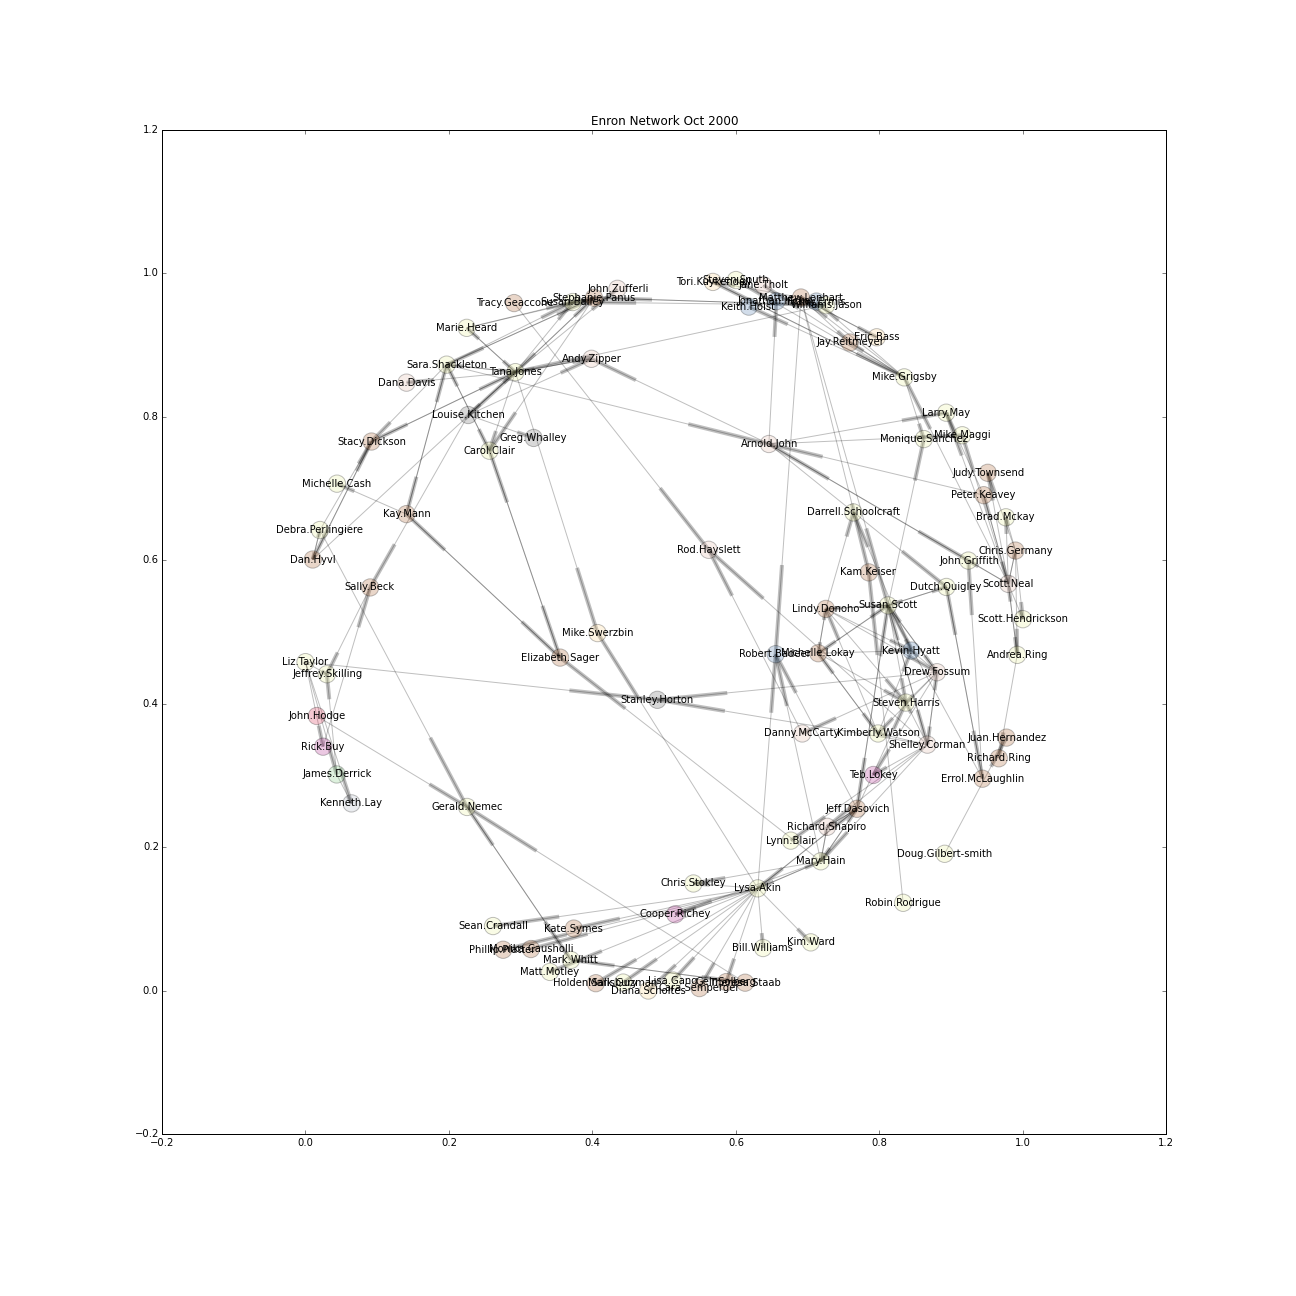
\includegraphics[width=1\textwidth]{figureEnronOct2000}
	
	Compare the network in Oct 2000 to this network created from emails sent in October 2001 at which point the fraud at Enron has been exposed and Enron is nearing bankruptcy.
	
	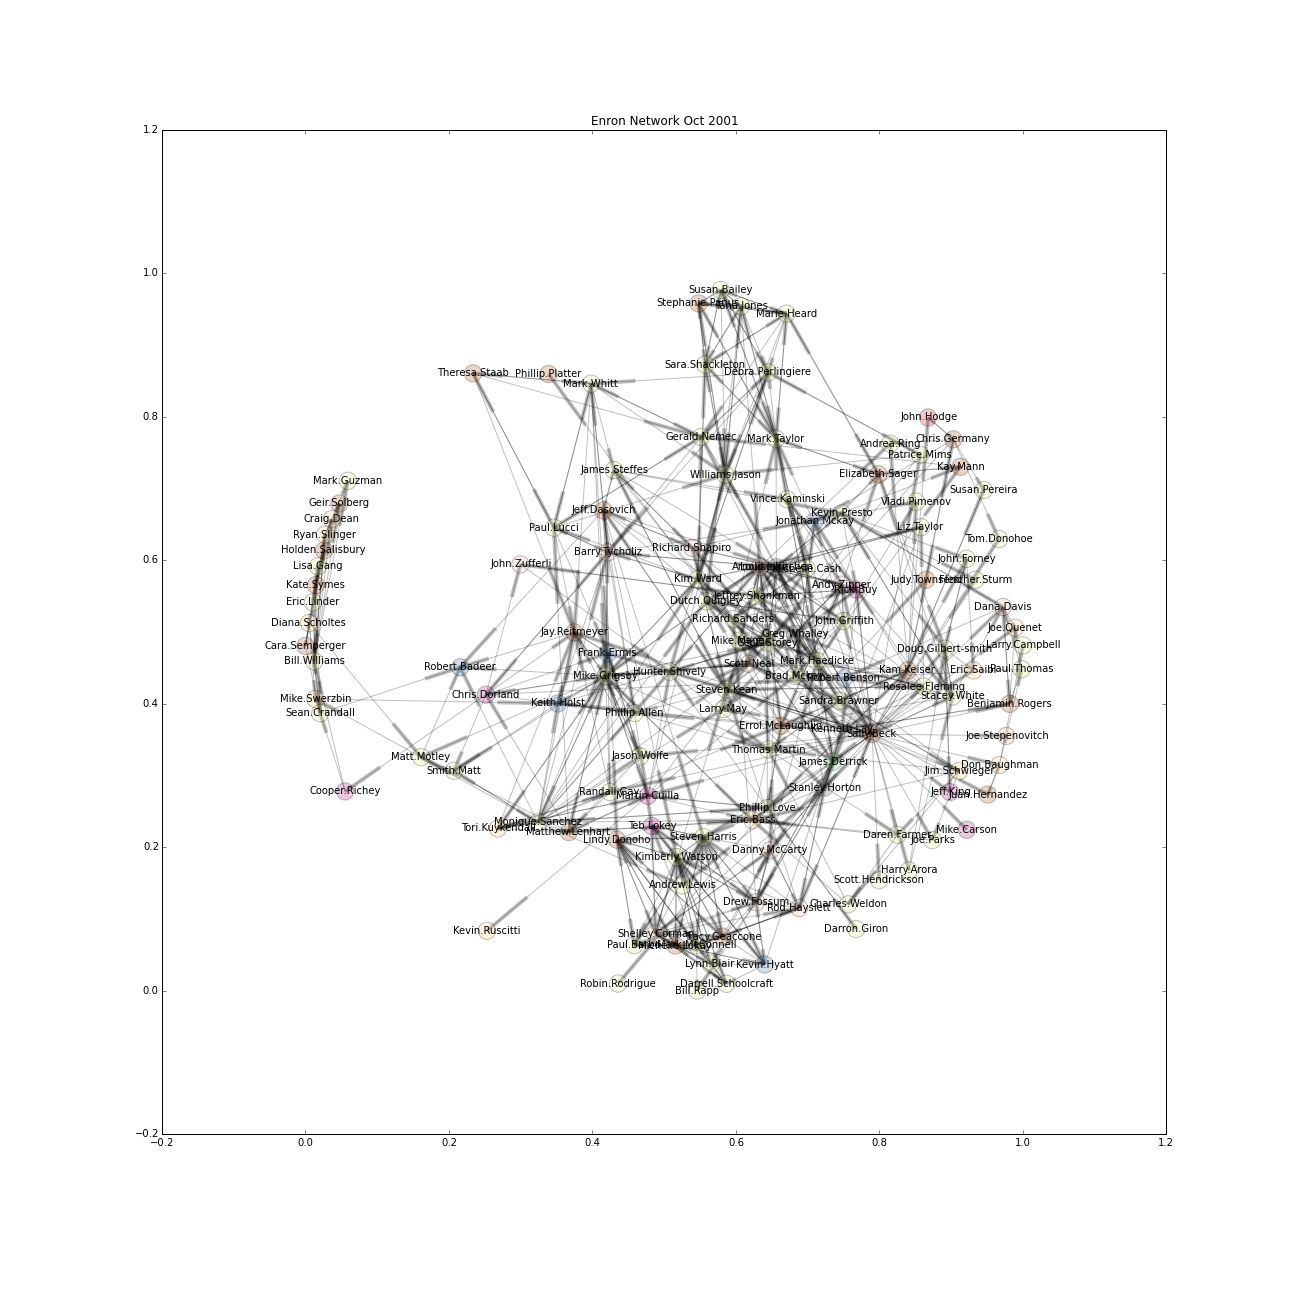
\includegraphics[width=1\textwidth]{figureEnronOct2001}
	
	\subsection{Terminology}
	\begin{enumerate}
		\item $A$ is the adjacency matrix of the network which is $n$ x $n$ for a network with $n$ nodes.
		\item $D$ is the diagonal matrix containing node degrees on it's diagonals
		\item $L$ is the laplacian of the matrix defined as $D - A$
		\item $B$ Is the modularity matrix defined as $B_{ij} = A_{ij} - \frac{k_i k_j}{2m}$ where $k_a$ is degree of node $a$
	\end{enumerate}

\section{Centrality Measures} One of the key questions one can ask about an information network such as the Enron email network is: Who are the most important actors in the network? There are various measures of centrality one can use to answer that question.	
	\subsection{Eigenvector Centrality} Eigenvector based centrality measures are based on the idea that a node is important if it is connected to other important nodes. Let $A$ be the adjacency matrix of a graph and $x$ the vector of centrality measures. We would like the centrality of each node to be proportional to the centralities of all the nodes connected to it. In matrix form then we would like vector $x$ to satisfy the 
		\begin{equation}
			A x = \kappa x
		\end{equation}
		Thus $x$ is an eigenvector of the matrix $A$. Even though all eigenvectors of $A$ satisfy the above equation, the eigenvector corresponding to the largest eigenvalue is used in practice. In order to compute the largest eigenvalue we use the power method.
		
        \begin{table}[h]
        \caption{Employees with Greatest Eigenvector Centrality}
        \centering
        \begin{tabular}{|l|l|l|}
        \hline
        \textbf{Name }          & \textbf{Eigenvector Centrality} & \textbf{Position}                              \\ \hline
        Sally Beck     & 0.238627               & Chief Operating Officer               \\ \hline
        Liz Taylor     & 0.229042               & Administrative Assistant to President \\ \hline
        Louise Kitchen & 0.220102               & President of Enron Online             \\ \hline
        Kenneth Lay    & 0.205464               & CEO                                   \\ \hline
        John Lavorato  & 0.201416               & CEO, Enron America                    \\ \hline
        Mike Grigsby   & 0.156134               & Vice President                        \\ \hline
        Kevin Presto   & 0.148424               & Vice President                        \\ \hline
        Scott Neal     & 0.147877               & Vice President, trader                \\ \hline
        Barry Tycholiz & 0.145584               & Vice President                        \\ \hline
        Arnold John    & 0.145032               & Vice President                        \\ \hline
        \end{tabular}
        \end{table}
	
	Katz centrality and PageRank are small modifications on the idea of eigenvector centrality. This measure identifies several key members of upper management at Enron despite the fact that they don't send or receive a lot of email.
	
	\subsection{Other measures of Centrality}
	
	\subsubsection{Closeness Centrality} This is defined as reciprocal of sum of shortest path distances from v to all other nodes. The closer a node is to others, the greater its centrality.

        \begin{table}[h]
        \caption{Employees with Greatest Closeness Centrality}
        \centering
        \begin{tabular}{|l|l|l|}
        \hline
        \textbf{Name} & \textbf{Closeness Centrality} & \textbf{Position}                     \\ \hline
        Liz Taylor        & 0.653509                      & Administrative Assistant to President \\ \hline
        Sally Beck        & 0.626050                      & Chief Operating Officer               \\ \hline
        John Lavorato     & 0.618257                      & CEO, Enron America                    \\ \hline
        Louise Kitchen    & 0.598394                      & President of Enron Online             \\ \hline
        Kenneth Lay       & 0.579767                      & CEO                                   \\ \hline
        Jeff Dasovich     & 0.541818                      & Executive, Government Relations       \\ \hline
        Kevin Presto      & 0.528369                      & Vice President                        \\ \hline
        Susan Scott       & 0.526502                      & Assistant Trader                      \\ \hline
        Mike Grigsby      & 0.520979                      & Vice President                        \\ \hline
        Arnold John       & 0.520979                      & Vice President                        \\ \hline
        \end{tabular}
        \end{table}
        
	\subsubsection{Betweenness Centrality} Betweenness centrality of a node is the sum of the fraction of all-pairs shortest paths that pass through that node.
	        
        \begin{table}[h]
        \caption{Employees with Greatest Betweenness Centrality}
        \centering
        \begin{tabular}{|l|l|l|}
        \hline
        \textbf{Name}  & \textbf{Betweenness Centrality} & \textbf{Position}                       \\ \hline
        Louise Kitchen & 0.100766                        & President of Enron Online               \\ \hline
        Susan Scott    & 0.069708                        & Assistant Trader                        \\ \hline
        Mike Grigsby   & 0.060098                        & Vice President                                        \\ \hline
        Kenneth Lay    & 0.048120                        & CEO                                     \\ \hline
        Kim Ward       & 0.046483                        & Associate Director, Enron North America \\ \hline
        Jeff Dasovich  & 0.045877                        & Executive, Government Relations         \\ \hline
        Liz Taylor     & 0.043397                        & Administrative Assistant to President   \\ \hline
        Sally Beck     & 0.043037                        & Chief Operating Officer                 \\ \hline
        Kevin Presto   & 0.040577                        & Vice President                          \\ \hline
        Bill Williams  & 0.037401                        & Trader                                  \\ \hline
        \end{tabular}
        \end{table}

\section{Communities} The basic goal of community detection is to separate the network into groups of vertices that have few connections between them. The following discussion is based on Mark Newman's work \cite{newman}. 

	
	Cut size is a simple metric that can be used to find communities in a network. The cut size is simply the number of edges you have to remove from the network so that the two groups of nodes become disconnected. 
	\begin{equation}
		R = \frac{1}{2} \sum_{i,j in different groups} A_{ij}
	\end{equation}
	where the factor of $\frac{1}{2}$ compensates for the fact that each edge appears twice in the adjacency matrix.

	Modularity is another (arguably better) measure. The idea is that we find  the fraction of edges that run between vertices of the same type, and then we subtract from that figure the fraction of such edges we would expect to find if edges were positioned at random without regard for vertex type \cite{networkBook}. When the fraction of edges between vertices of the same type is significantly greater than what would be expected at random, we can say that the network exhibits high homophily. The number of edges that run between nodes of the same type is given by
	\begin{equation}
		\sum_{edges (i,j)} \delta (c_i, c_j) = \frac{1}{2} A_{ij} \delta (c_i, c_j)
	\end{equation}
	where $c_i$ and $c_j$ are the classes of nodes and $\delta (m,n)$ is the Kronecker delta which is equal to 1 if $m = n$ and 0 otherwise.
	
	
	The expected number of edges between nodes of the same type is given by
	\begin{equation}
		\frac{1}{2} \sum_{i,j} \frac{k_i k_j}{2m} \delta (c_i,c_j)
	\end{equation}
	where $k_i$ denotes the number of edges of node $i$ (it's degree) and $m$ is the total number of edges in the network. Subtracting (3) from (2) gives us modularity $Q$
	\begin{equation}
		Q = \frac{1}{2m} \sum_{i,j} \left( A_{ij} - \frac{k_i k_j}{2m} \right) \delta (c_i,c_j)
	\end{equation}

	\subsection{Partitioning using Cut Size} 
	We can use these ideas to find communities within a network.  
	
	Let us define quantities $s_i$ for each vertex $i$, which represent the division of the network: 
	\begin{align}
		s_i = +1 \text{ if node belongs in group 1} \\
		s_i = -1 \text{ if node belongs in group 2}
	\end{align}
	Then
	\begin{align}
		\frac{1}{2} (1 - s_i s_j) = 1 \text{ if i and j are in the same group} \\
		\frac{1}{2} (1 - s_i s_j) = 0 \text{ if i and j are in different groups}
	\end{align}
	
	This allows us to rewrite equation 2 for cut size as
	\begin{equation}
		R = \frac{1}{4} \sum_{ij} A_{ij} (1- s_i s_j)
	\end{equation}
	
	Simplifying the above equation and using the fact that $\sum_j A_{ij} = k_i$ we get
	\begin{equation}
		R = \frac{1}{4} \sum_{ij} (k_i \delta_{ij} - A_{ij}) s_i s_j = \frac{1}{4} \sum_{ij} L_{ij} s_i s_j
	\end{equation}
	where $L$ is the Laplacian of the matrix. We can rewrite this equation in matrix form as 
	\begin{equation}
		R = \frac{1}{4} s^T L s
	\end{equation}
	where $s$ is the vector of all $s_i$. Equation 12 gives us a optimization problem: find $s$ such that the quantity $R$ is minimized. $s$ is constrained to only have values that are +1 or -1. \\
	
	This turns out to be a very difficult problem to solve so we relax some of the constraints on $s$. $s$ is allowed to take any value subject to $|s|$ = $\sqrt{n}$ where $n$ is the number of nodes and $1^T s = n_1 - n_2 $ where $n_1$ and $n_2$ are the sizes of the partitions we need. 
	
	We can differentiate with respect to $s$ and introduce two Lagrange multipliers to solve this problem
	\begin{equation}
		\frac{\partial}{\partial s_i} 
			\left[ 
			\sum_{jk} L_{jk} s_j s_k 
			+ \lambda \left( n - \sum_j s_j^2 \right)
			+ 2 \mu \left( (n_1 - n_2) - \sum_i s_j \right)
			\right] = 0 
	\end{equation}
	
	This results in
	\begin{equation}
		L s = \lambda s + \mu 1 
	\end{equation} \\
	
	It is easy to see that the vector 1 is an eigenvector of a Laplacian matrix since the sum of the off-diagonal entries of a Laplacian is the degree which is 0 minus the diagonal element of the matrix. Knowing this allows us to compute $\mu = - \frac{n_1 - n_2}{n} \lambda$. \\
	
	If we define a new vector $x$ = $s + \frac{\mu}{\lambda} 1$ we can see that $L x = \lambda x$. We now need to pick a $\lambda$ such that $R$ (the cut size) is minimized. Solving for $R$ we get
	\begin{equation}
		R = \frac{n_1 n_2}{n} \lambda
	\end{equation}
	
	The cut size is thus proportional to the eigenvalue $\lambda$. Given that we want to minimize $R$ we should choose $\lambda$ to be the smallest eigenvalue of $L$. But we know that all the eigenvalues of $L$ are non-negative and the smallest of them is the 0 vector.  So the best option is to choose the eigenvector $v_2$ corresponding to the second lowest eigenvalue $\lambda_2$ of the Laplacian matrix. 

	Applying this technique to the Enron network to try to split it into roughly equal halves we get the following using data from October 2001
	
	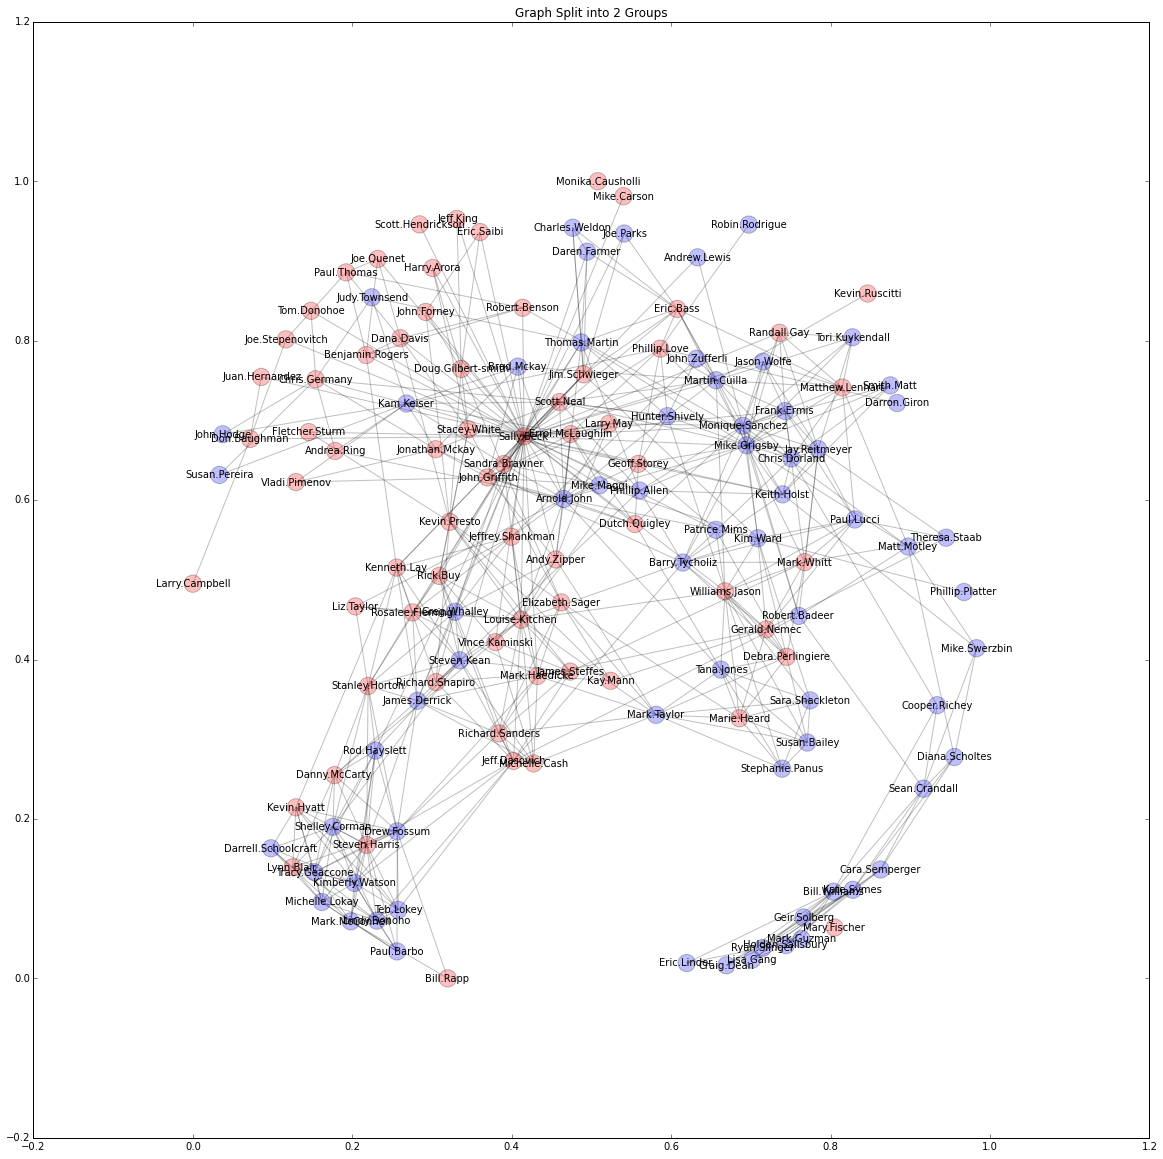
\includegraphics[width=1\textwidth]{figureEnronPartition}
	
	The modularity of this division is 0.16. As previously mentioned a positive number means there is homophily in the network. 
	
	\subsection{Modularity Maximization Using Spectral Techniques} 
	We can also use the idea of modularity to find communities within a network. As discussed earlier modularity is defined as 
	\begin{equation}
		Q = \frac{1}{2m} \sum_{i,j} \left( A_{ij} - \frac{k_i k_j}{2m} \right) \delta (c_i,c_j)
	\end{equation}
	or
	\begin{equation}
		Q = \frac{1}{2m} \sum_{i,j} B_{ij} \delta (c_i,c_j)
	\end{equation}
	\\
	We set up a vector $s$ in the same fashion as we did in the previous section so that $\delta (c_i,c_j)$ = $\frac{1}{2} (s_i s_j + 1)$. Substituting that back into the definition of modularity we get
	\begin{equation}
		Q = \frac{1}{4m} s^T B s
	\end{equation}
	This equation is once again of a similar form as the cut size equation in the previous section. 
	\\
	To solve this optimization problem we once again relax the constraint on $s$ to only take values of +/- 1 and allow $s$ to be any number subject to $|s|$ = $\sqrt{n}$. Differentiating with respect to the elements of $s$ and introducing a Lagrangian we get
	\begin{equation}
		\frac{\partial}{\partial s_i} 
			\left[ 
			\sum_{jk} B_{jk} s_j s_k 
			+ \beta \left( n - \sum_j s_j^2 \right)
			\right] = 0
	\end{equation}
	which ultimately gives
	\begin{equation}
		B s = \beta s
	\end{equation}
	\\
	In other words $s$ is an eigenvector of $B$. Substituting back into the equation for modularity you get
	\begin{equation}
		Q = \frac{n}{4m} \beta
	\end{equation}
	since $s^T s = n$
	\\
	
	In this case we want to maximize modularity so we need to pick $s$ accordingly. If $u_1$ is the eigenvector corresponding to the largest eigenvalue then we need to maximize $s^T u_1$. The best we can do is make each term in $s^T u_1$ positive. So if $u_{1_i}$ is negative we set $s_i$ to be -1 and +1 otherwise. This give us a relatively simple algorithm whereby we only need to look at the sign of each element of the eigenvector corresponding to the largest eigenvalue of the modularity matrix to find partitions in the data. 
	
	This technique can also be applied repeatedly to divided the network into more than two partitions. Applying this technique to the Enron network using data from October 2001 we get
	
	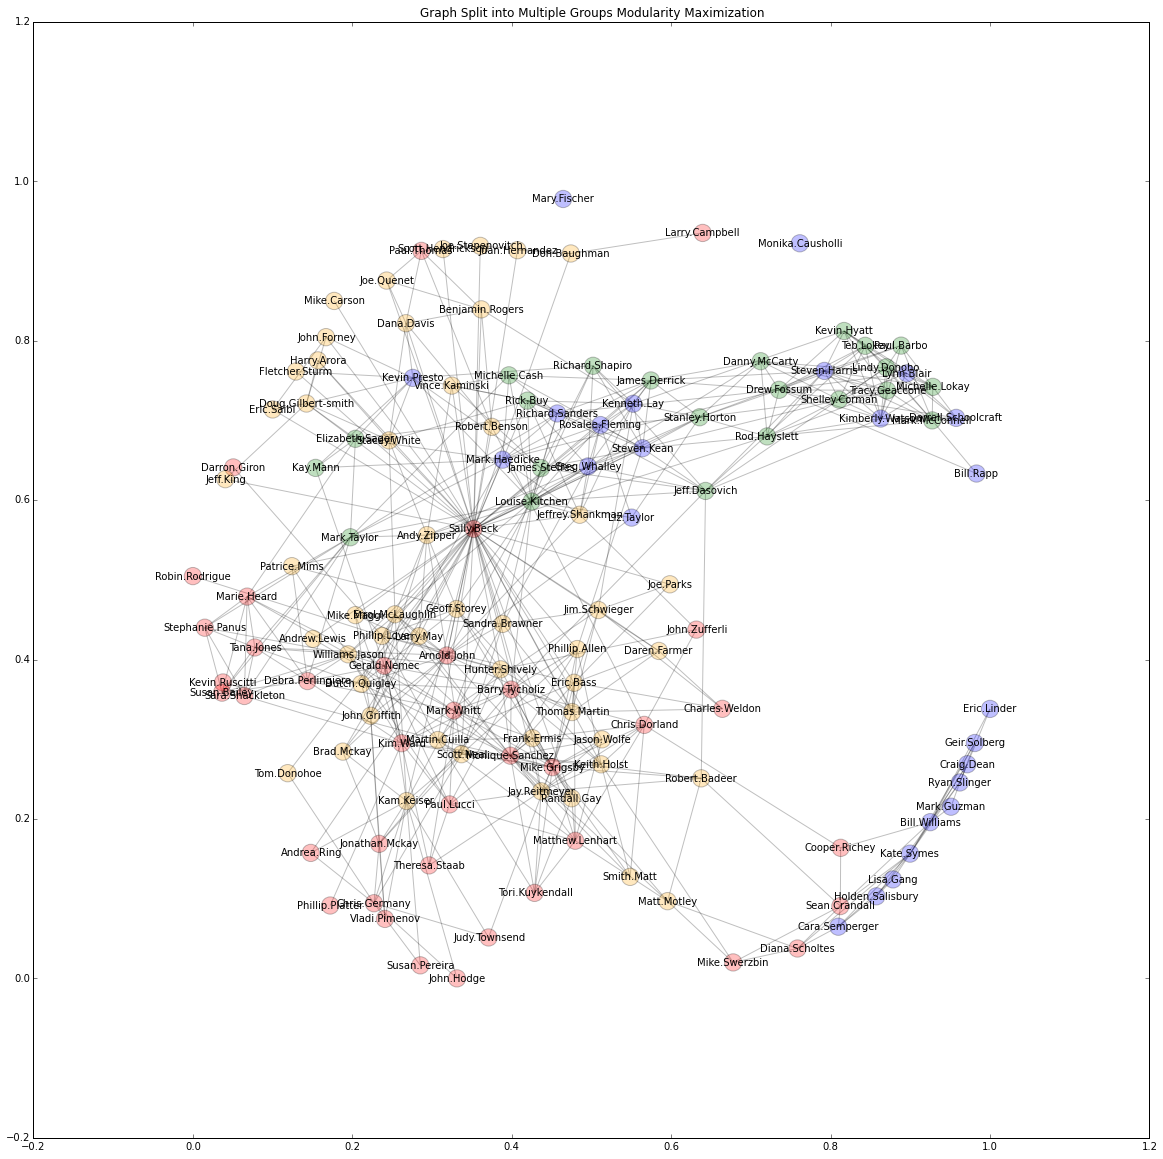
\includegraphics[width=1\textwidth]{figureEnronPartitionMult}



	\subsection{Singular Value Decomposiiton}
		We can look at singular values of the adjacency matrix to obtain low rank approximations of the network and find communities within the network. 
		

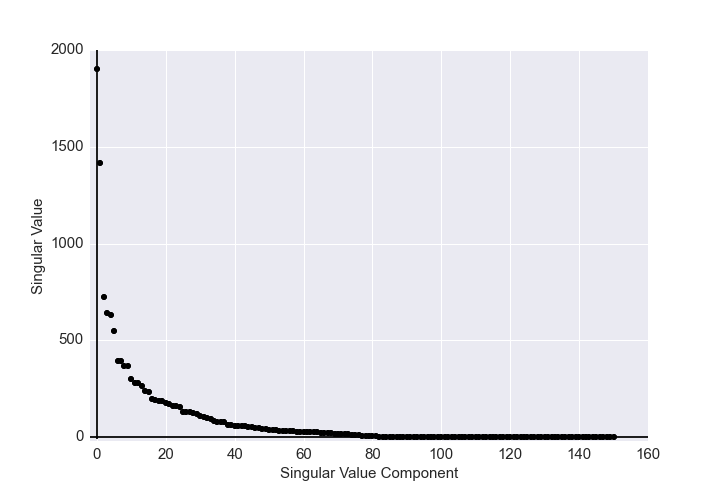
\includegraphics[width=1\textwidth]{SingularValues}


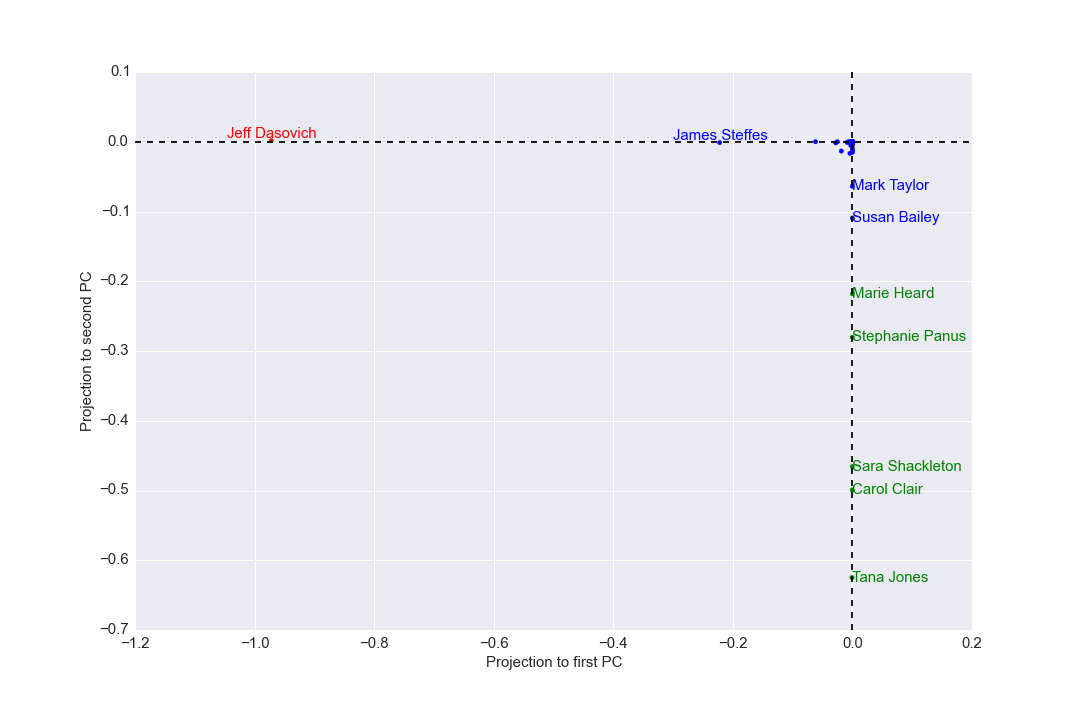
\includegraphics[width=1\textwidth]{ProjectionPC}


%\begin{figure*}[t!]
%    \centering
%    \begin{subfigure}[t]{0.5\textwidth}
%        \centering
%        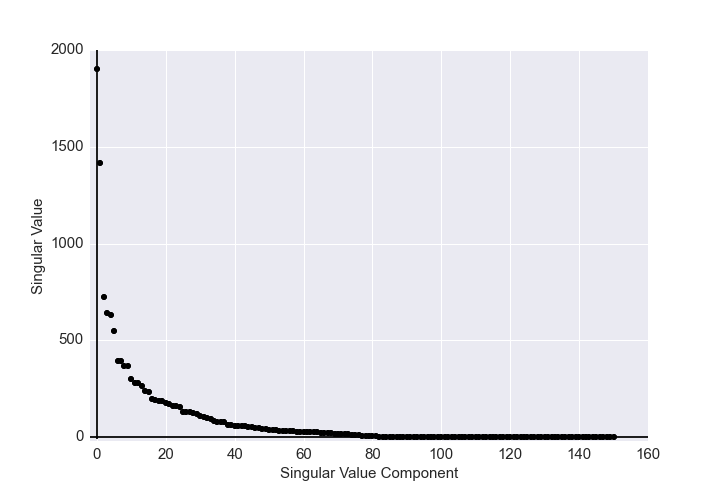
\includegraphics[height=1.2in]{SingularValues}
%        \caption{Singular values of the adjacency matrix}
%    \end{subfigure}
%    \begin{subfigure}[t]{0.5\textwidth}
%        \centering
%        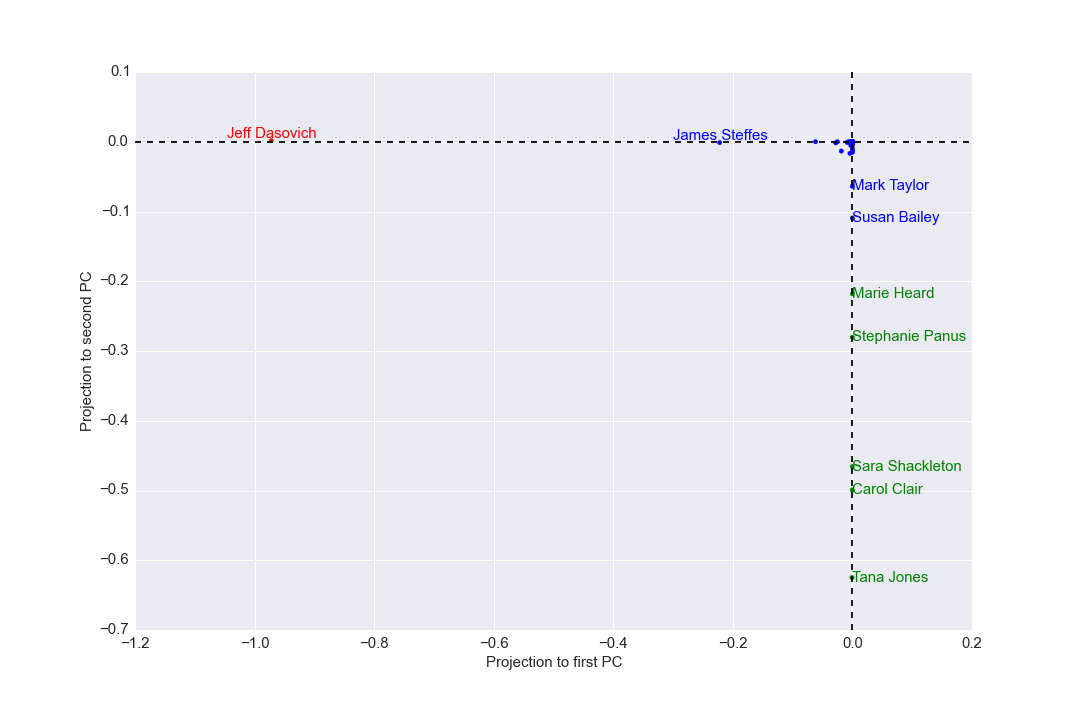
\includegraphics[height=1.2in]{ProjectionPC}
%        \caption{Employee projection to the principal components}
%    \end{subfigure}
%    \caption{Caption place holder}
%\end{figure*}


\section{Evolution Across Time} The Enron network was obviously an evolving network over time. This longitudinal information allows us to study how the network changed over time across various dimensions. We show a few of them below.


%\begin{figure}[H]
%\centering
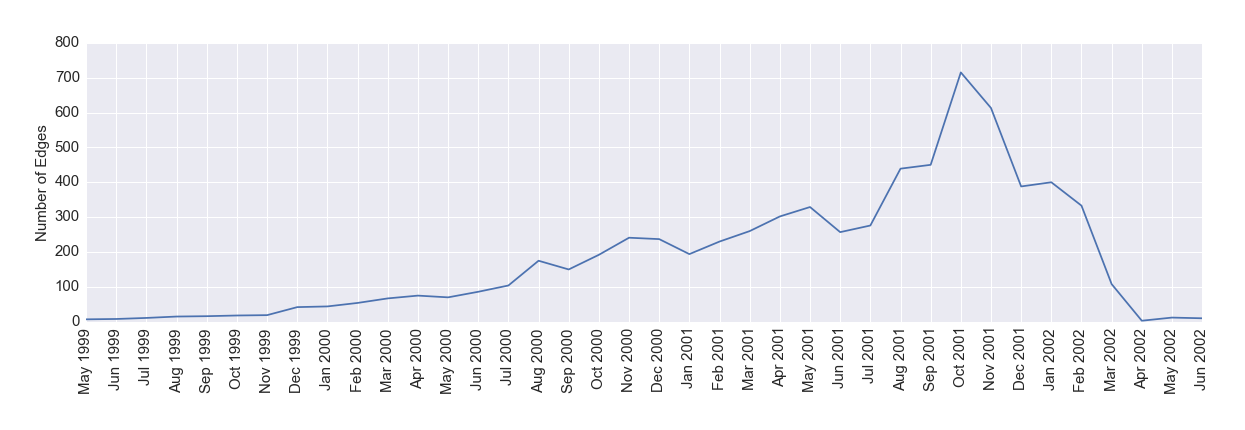
\includegraphics[width=1\textwidth]{Timeseries_Edges}
%\caption{Number of edges in the network through time}
%\end{figure}

%\begin{figure}[ht]
%\centering
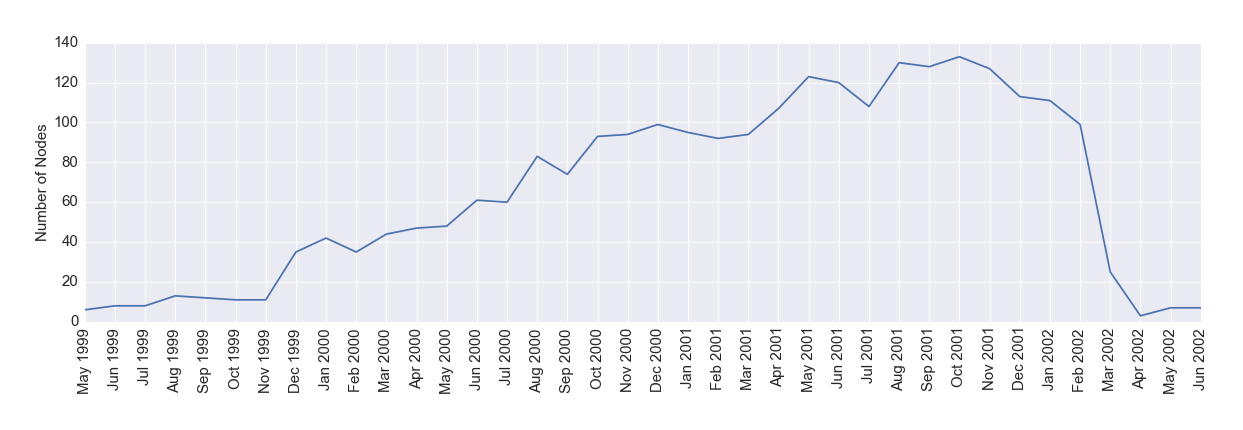
\includegraphics[width=1\textwidth]{Timeseries_Nodes}
%\caption{Number of nodes in the network through time}
%\end{figure}

%\begin{figure}[ht]
%\centering
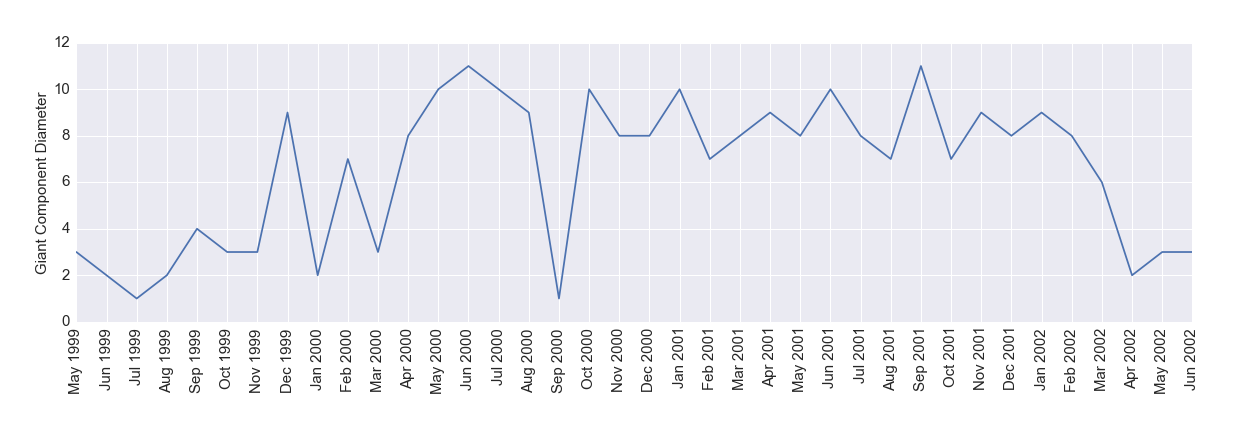
\includegraphics[width=1\textwidth]{Timeseries_GiantDiameter}
%\caption{Size of the giant component diameter}
%\end{figure}

%\begin{figure}[ht]
%\centering
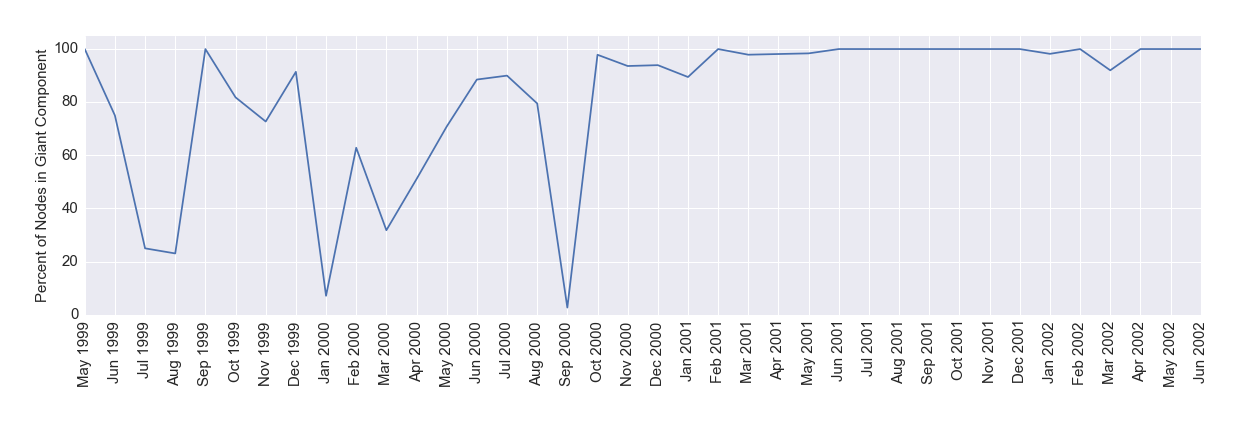
\includegraphics[width=1\textwidth]{Timeseries_GiantSize}
%\caption{Percent of nodes connected to the giant component}
%\end{figure}

%\begin{figure}[ht]
%\centering
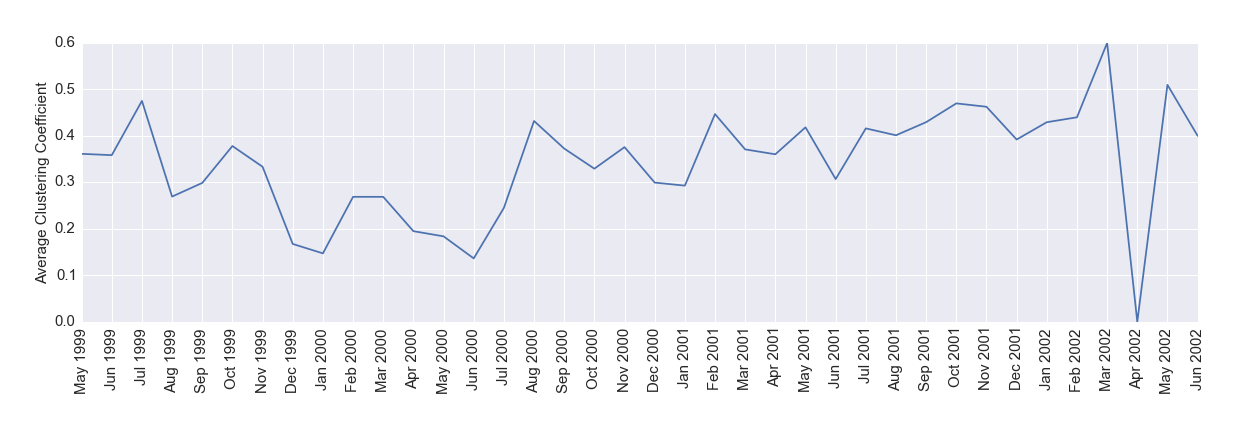
\includegraphics[width=1\textwidth]{Timeseries_ClusteringCoefficient}
%\caption{Average clustering coefficient of the network }
%\end{figure}

%\begin{figure}[ht]
%\centering
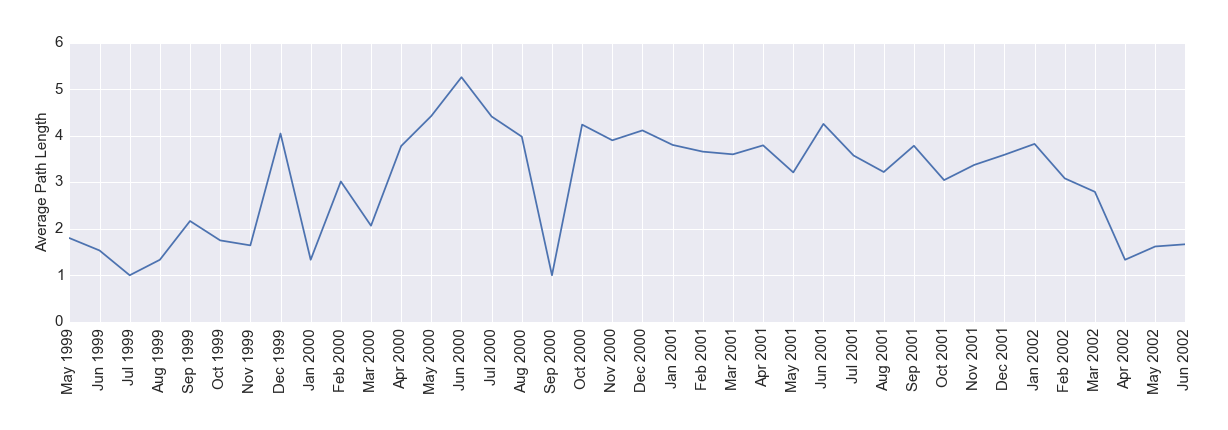
\includegraphics[width=1\textwidth]{Timeseries_PathLength}
%\caption{Average path length}
%\end{figure}

%\begin{figure}[ht]
%\centering
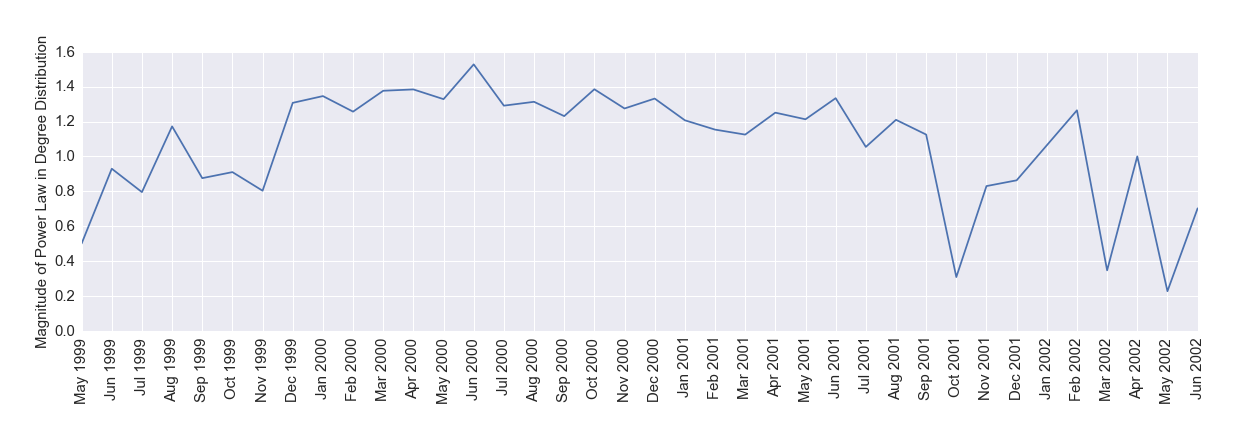
\includegraphics[width=1\textwidth]{Timeseries_PowerLaw}
%\caption{Power law exponent of degree distribution }
%\end{figure}

\section{Conclusions}
	We were able to identify key actors at Enron by simply analyzing the data rather than looking at complicated organizational charts. While some people (like the CEO Ken Lay) are expected to be central members of the company, certain other people might have been overlooked. Network analysis can help identify those people. It is quite strange for Jeff Dasovich, a governmental relations executive, to be a central member of this network.
	
	This analysis also helps find communities within the network. Interpreting these groups of people might require specific knowledge about the company but it can help unearth connections between people that might have been missed.
	
	Longitudinal analysis of this data allows us to see that the network gets increasingly dense over time as the crisis at Enron balloons. This might help us understand the nature of organizations under duress. 

\begin{thebibliography}{9}

\bibitem{shetty}
Shetty, J., Adibi, J. (n.d.). The Enron Dataset
Database Schema and Brief Statistical Report

\bibitem{pfeiffer}
https://www.cs.purdue.edu/homes/jpfeiff/enron.html
data retrieved on Nov 11 2014

\bibitem{nyt}
http://www.nytimes.com/2006/01/18/business/worldbusiness/18iht-web.0117enron.time.html

\bibitem{park}
http://cis.jhu.edu/~parky/Enron/employees

\bibitem{newman}
Networks: An Introduction by M.E.J Newman


\end{thebibliography}


\end{document}
